\documentclass{standalone}
\usepackage{tikz}
% default colors
% used in standalone pictures and when no university is selected
\definecolor{black}{HTML}{000000}
\definecolor{green}{HTML}{33BB33}
\definecolor{red}{HTML}{BB3333}
\definecolor{orange}{HTML}{BB6600}
\definecolor{blue}{HTML}{3333BB}
\definecolor{uulmaccent}{HTML}{999999}

\definecolor{uulmlogoblue}{named}{blue}
\definecolor{uulmblue}{named}{blue}

\ifdarkmode
	\colorlet{green}{green!85!white}
	\colorlet{red}{red!85!white}
	\colorlet{orange}{orange!85!white}
	\colorlet{blue}{blue!85!white}
	\setbeamercolor{section in toc shaded}{fg=black}
	\setbeamertemplate{section in toc shaded}[default][50]
\fi


\begin{document}
	\sffamily
	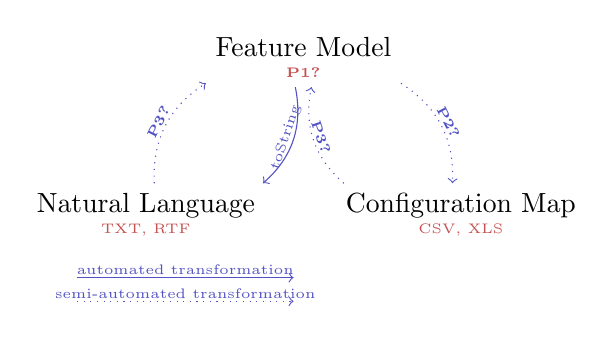
\begin{tikzpicture}
		\tikzstyle{every edge}=[font=\tiny,draw,color=blue]
		\node (fd) at (2,0) [align=center] {Feature Model\\[-1ex]{\tiny\color{red}\textbf{P1?}}};
		\node (nat) at (0,-2) [align=center] {Natural Language\\[-1ex]{\tiny\color{red}TXT, RTF}};
		\node (cfg) at (4,-2) [align=center] {Configuration Map\\[-1ex]{\tiny\color{red}CSV, XLS}};

		\path [->] (fd) edge[bend left] node[sloped,yshift=1mm] {toString} (nat);
		\path [dotted, ->] (nat) edge[bend left] node[sloped,yshift=1mm] {\textbf{P3?}} (fd);
		
		\path [dotted, ->] (fd) edge[bend left] node[sloped,yshift=1mm] {\textbf{P2?}} (cfg);
		\path [dotted, ->] (cfg) edge[bend left] node[sloped,yshift=1mm] {\textbf{P3?}} (fd);

		\node (trans) at (-1,-2.8) {};
		\node (trans2) at (2,-2.8) {};
		\node (trans3) at (-1,-3.1) {};
		\node (trans4) at (2,-3.1) {};
		\path [->] (trans) edge node[yshift=1mm] {automated transformation} (trans2);
		\path [dotted, ->] (trans3) edge[yshift=5mm] node[yshift=1mm] {semi-automated transformation} (trans4);
	\end{tikzpicture}
\end{document}